%% aps to author template--please use pdflatex to edit then to pdf--------------
\documentclass[A4,twoside,fontset=ubuntu,UTF8]{ctexart}
%\usepackage{slashbox}\usepackage{makecell}\usepackage{diagbox}\backslashbox
\usepackage{aappss}
\usepackage{subcaption}
\usepackage{tabularx}
%\usepackage{epstopdf}

\newcommand{\vx}{{\mathbf{x}}}
%\renewcommand\baselinestretch{1.235}\protect
\renewcommand\baselinestretch{2.0}\protect
\newcommand{\bigO}{{\mathcal{O}}}
\newcommand{\ra}[1]{\renewcommand{\arraystretch}{#1}}
\abovedisplayshortskip 0 pt plus 3pt
\belowdisplayshortskip 6 pt plus 2pt minus 2pt
\abovedisplayskip 6 pt plus 2pt minus 2pt
\belowdisplayskip 6 pt plus 2pt minus 2pt
% \info{2015}{64}{1}{01{}} \infodate{2015.0.0.}{2015.0.0.}
%=================== Text begin here ==============================
\begin{document}\apsname

\title{自动微分数值计算理论-地震波模拟为例 \fivestar}%{\cfundlink}

\author{刘金国$^{1)}$ \quad 许开来$^{2)}$}

\address{1)}{哈佛大学物理系, 坎布里奇 \quad 02138}
\address{2)}{斯坦佛大学, 斯坦佛 \quad 94305}

%\address{3)}{}

\abstract{自动微分是机器学习中核心的数值技术,它被用于高效,自动的对程序求导。
如今越来越多的物理学者意识到高效,自动的求导可以对很多物理问题的求解提供新的思路。
本文介绍自动微分技术相关的主要理论,并以地震波的模拟为例介绍它的应用。}

\keywords{自动微分,科学计算,编程语言}

% https://ufn.ru/en/pacs/all/
% 02.60.Pn numerical optimization
% 02.30.Jr Partial differential equations
\pacs{02.60.Pn, 02.30.Jr}

\cfund{}

\cmail{jinguoliu@g.harvard.edu \quad }

%\cmailddag{mail2}

%\mail{}{}\cmail \cmailddag

%\apscopyright \baselineskip=16.0pt plus.2pt minus.2pt
%\begin{multicols}{2}\sec
\vskip 0.55\baselineskip
\section{引~~~~言}
    自动微分是指自动获取一个目标计算机程序导数的技术。很多人了解它是因为它在机器学习中的成功应用,人们可以用它优化带有千亿参数的神经元网络~\cite{Rosset2019}。
与很多人印象不同的是,自动微分其实是个很古老的技术。
Nolan曾在他1953年的博士论文中就提出过~\cite{Nolan1953}自动化求导计算机程序的构想,
而最近十几年,自动微分在科学计算中的应用越来越广泛并拓展了人们可解决问题的范畴。
%过去人们需要依赖手动推导求解导数,也因此限制了一个算法可处理问题的范围。
    一个典型的例子是变分蒙特卡洛算法。
过去,人们会将变分基态假设为Gutzwiller波函数~\cite{Gutzwiller1963}这样具有良好解析性质的函数。
直到2017年,Carleo等人~\cite{Carleo2017, Deng2017}把机器学习中的一些变分模型限制波尔兹曼机(RBM)带入到了大家的视野。由于RBM的解析性质很好,计算所需的求导过程可以通过解析推导,所以当时人们并没有强烈的利用计算机辅助求导的动机。
但受此启发,大家意识到不光是RBM这样解析性质好的函数,任何机器学习中的神经元网络也可以被用做波函数的猜测形式~\cite{Cai2018}。
而且如果可以用流行的机器学习框架,比如脸书公司开发的PyTorch和谷歌公司开发的TesnorFlow来编写生成波函数的代码,人们可以避免手动推导导数的麻烦,从而可以把波函数的表达变得更加自由。
而现在,随着人们对微分的认知更加深刻,波函数不光可以表达为以张量运算为主体的神经元网络,还可以是几乎任意的计算机程序。
%一段通用的代码总可以被分解成一些加减乘除这样的基础解析函数,知晓基础函数的自动微分规则,计算机可以通过链式法则用计算机推导出整个程序的导数。
    除了这个例子,科学家们利用方便的,自动化的计算机辅助求导还解决了很多包括量子模拟~\cite{Luo2019},张量网络~\cite{Liao2019},组合优化~\cite{Liu2020},海洋学~\cite{Heimbach2005}和地震学~\cite{Symes2007,Zhu2020}等领域中的问题。
甚至是一些非解析的蒙特卡洛抽样过程,人们也设计出了一些办法对其自动化的求导~\cite{Zhang2019}。

那物理学家们是否只需要奉行“拿来主义”,仅阅读机器学习库的文档,就可以很好的驾驭自动微分呢?
并不完全是的,当大家谈论自动微分的时候有“狭义”和“广义”之分,而主流机器学习库仅涵盖了前者。
这里狭义自动微分是指机器学习库中广泛应用的以张量为基本数据类型的自动微分。它通过对常用的函数族(矩阵乘法,卷积函数,relu函数等)手动定义导数后向传递的规则,并通过链式法则将它们连接起来得到程序的导数。
手动定义常用函数导数可以对函数有更加针对性的优化从而保证张量运算的性能,但缺点是,它往往无法满足科学计算的研究中对函数求导的多元化需求。有些时候人们可以通过手动添加一些求导规则来辅助求导,比如在张量网络等模拟中需要用到的复数奇异值分解函数~\cite{Wan2019,Liao2019}。
但是也有一些时候添加求导规则也无济于事,比如,严格对教化求解基态过程中用到的极大极小本正值求解器~\cite{Xie2020}和模拟变分量子算法中幺正量子线路的求导~\cite{Luo2019}的求导,前者涉及了无法表达为向量函数的稀疏矩阵的构造过程而后者涉及了利用可逆性回溯中间状态。
还有些时候手动定义的导数可能会出错,尤其是将定义在实数上的规则拓展到复数域的时候。比如奇异值分解函数的求导规则直到2019年,才有人意识到复数的求导规则中有一个规范不变性带来的一项被忽略了~\cite{Wan2019}。
而广义的自动微分没有这些问题,它微分规则定义在标量的最基础的运算之上,这些基础运算有限而且很难出错。
    一个很好的描述它与狭义自动微分区别的例子是,当将两个复数相加,广义的自动微分看到的是实部相加和虚部相加这两个操作,而狭义自动微分则需要推导适用于复变函数的Wirtinger导数~\cite{Hirose2003}。
但广义自动微分的强大威力同时也带来了一些问题,其中最核心的问题是广义的后向自动微分把机器学习中本身就存在的内存占用问题扩大了,
使得用户不得不直接或间接的面对这些问题。
为了让研究者们更好的利用自动微分解决物理中的实际问题,本文的向物理学家们介绍自动微分中的几种核心概念以及它在微分模拟地震波传播过程中的应用。
章节\ref{sec:forwardbackward}~ 介绍了两种基本的自动微分模式,前向和后向自动微分。
章节\ref{sec:timespace}~ 介绍了基于检查点和可逆编程的两种广义后向自动微分的基础理论,尤其两者如何权衡程序的运行时间和空间。
章节\ref{sec:applications}~ 介绍了不同广义自动微分技术在微分地震波模拟过程中的应用。

\section{链式法则的两种传递方式}\label{sec:forwardbackward}

    自动微分可以分为两大类,一种叫做前向传播(Forward propagation)~\cite{Wengert1964},一种叫做后向传播(Backward propagation)~\cite{Boltyanski1960}。


%为了直观的理解它们的不同,这里考虑一个计算过程 $f : \mathbb{R}^m \rightarrow \mathbb{R}^n$
%\begin{align*}
    %&\vx^1 = f_1(\vx^0)\\
    %&\vx^2 = f_2(\vx^1)\\
    %&\ldots\\
    %&\vx^L = f_L(\vx^{L-1})
%\end{align*}
%其中 $x^0\in R^m$, $x^L\in R^n$, $L$是计算的步骤数。
%这段程序的雅可比 (Jacobian) 矩阵$J_{ij} \equiv \frac{\partial x^L_i}{\partial x_j^0}$是一个$n\times m$的矩阵,其中$x_j^0$和$x_i^L$代表了输入和输出中的一个元素。
%前向自动微分的链式法则表述为$\frac{\partial \vx^k}{\partial x^0_j} = \frac{\partial \vx^k}{\partial \vx^{k-1}}\frac{\partial \vx^{k-1}}{\partial x^0_j}$,它计算了雅可比矩阵的第$j$列。后向自动微分的链式法则为$\frac{\partial \vx^L_i}{\partial x^{k-1}} = \frac{\partial \vx^L_i}{\partial \vx^{k}}\frac{\partial \vx^{k}}{\partial x^{k-1}}$,它计算了雅可比矩阵的第$i$行。
%在大多数应用中,计算一行雅可比矩阵比计算一列有用的多,因为
%后向自动微分的实现难度远高于前向自动微分,因为它的梯度计算方向和计算本身的方向相反,如何回溯中间状态成了一个核心的问题。

    \begin{figure}[t]
\centering
\begin{subfigure}[b]{0.32\textwidth}
    \centering
    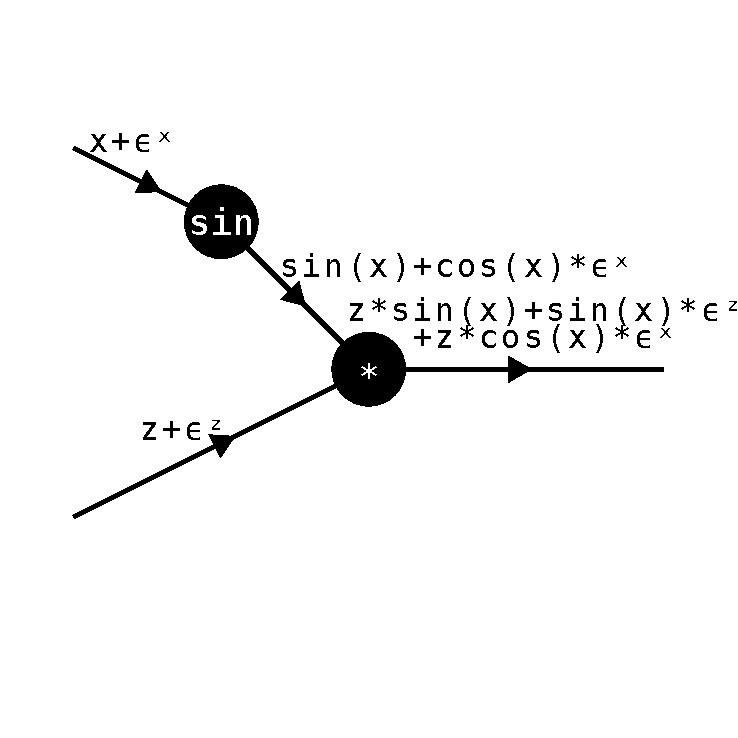
\includegraphics[width=\textwidth, trim={1cm 3cm 0cm 1cm}, clip]{./forwarddiff.pdf}
    \caption{\small 前向自动微分}
\end{subfigure}
\begin{subfigure}[b]{0.32\textwidth}
    \centering
    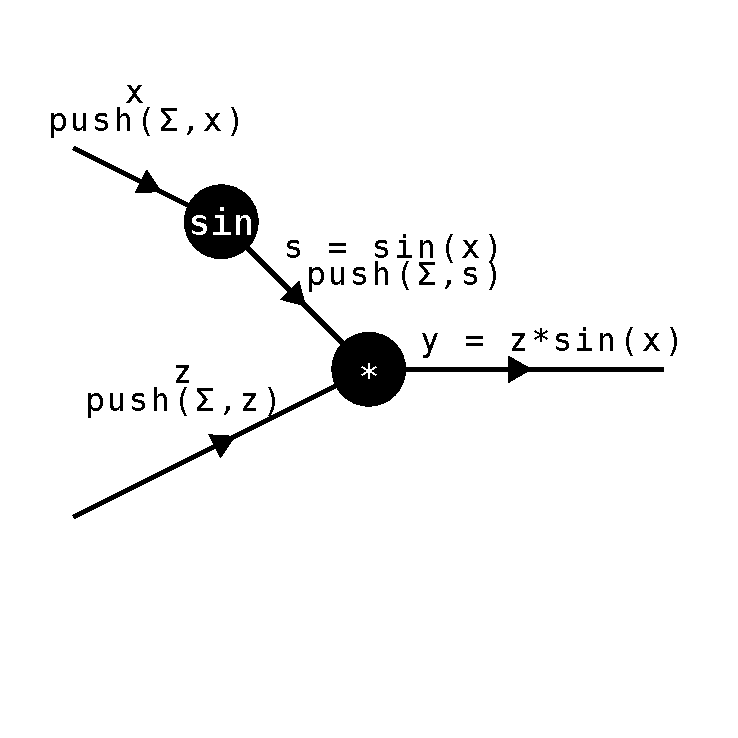
\includegraphics[width=\textwidth, trim={0 3cm 1cm 1cm}, clip]{./backward-forward.pdf}
    \caption{\small 后向自动微分中的前向计算}
\end{subfigure}
\begin{subfigure}[b]{0.32\textwidth}
    \centering
    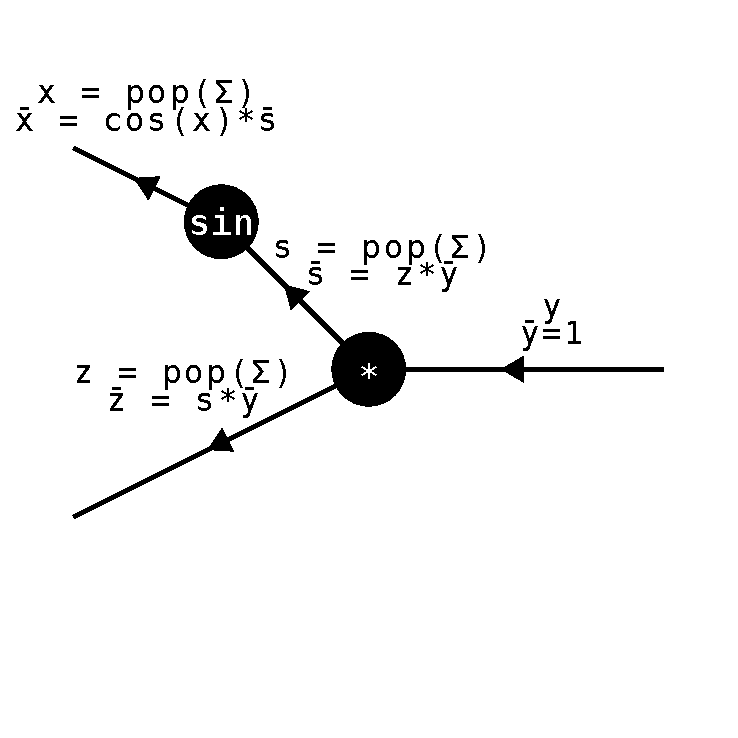
\includegraphics[width=\textwidth, trim={0 3cm 1cm 1cm}, clip]{./backward-backward.pdf}
    \caption{\small 后向自动微分中的梯度反向传播}
\end{subfigure}
        \caption{利用自动微分计算对于计算过程$y = z \sin(x)$的导数$\overline{x}\equiv \frac{\partial y}{\partial x}$和$\overline{z}\equiv \frac{\partial y}{\partial z}$。其中圆圈代表函数,线代表变量,箭头代表运算方向,$\Sigma$是一个用于缓存中间计算结果的全局堆栈而\texttt{push}和\texttt{pop}分别代表了对该堆栈的入栈和出栈操作。\label{fig:autodifftypes}} 
\end{figure}

让我们从图\ref{fig:autodifftypes}中演示的例子出发看看它们有何异同。(a)所示的是前向自动微分在运算中会携带一种特殊的变量$\epsilon^i$,它正是我们高等数学中的“无穷小量”,而上标$i$代表它对应第$i$个变量。
计算中我们只保留到一阶,因此它满足代数规则$\epsilon^i\epsilon^j = 0$。
前向自动微分作用在标量上的梯度的第推公式为
\begin{align}
    f(x+\sum\limits^k_{i=1} y_i \epsilon^i) = f(x) + \frac{\partial f(x)}{\partial x} \sum\limits^k_{i=1}y_i\epsilon^i
\end{align}

因此,实现一个前向自动微分本质就是实现一种携带无穷小量的特殊变量在函数作用下的变换。
前向自动微分的计算时间随着需求导的变量的数目线性增长。因为随着变量数目的增加,$\epsilon$的数目线性增加,函数的操作数也随之线性增加。
其中,$\epsilon^i$正是我们高等数学中的“无穷小量”,而下标$i$代表它对应第$i$个变量。计算中我们只保留到一阶,因此它满足代数规则$\epsilon^i\epsilon^j = 0$。因此,实现一个前向自动微分本质就是实现一种携带无穷小量的特殊变量在函数作用下的变换。
前向自动微分的计算时间随着需求导的变量的数目线性增长。因为随着变量数目的增加,$\epsilon$的数目线性增加,函数的操作数也随之线性增加。

图 (b) 和 (c) 展示了后向自动微分的前向过程和后向过程,前向过程中函数除了运算本身,还会将部分中间结果放入一个全局堆栈$\Sigma$中,
而后向过程将这些缓存的结果出栈并利用如下递推公式计算导数
\begin{align}
    \overline{x} = \frac{\partial f(x)}{\partial x}\overline{y}
\end{align}
其中,$\overline{\cdot}$代表了相应变量的梯度$\frac{\partial \mathcal{L}}{\partial \cdot}$,这个定义同时隐含了程序最终会输出一个标量$\mathcal{L}$作为损失函数。
这个算法的复杂度对于需要求导的变量数目不敏感,相反因为这里假设了输出变量只有一个,该算法的实际计算量会随着输出变量的数目而线性增加。但考虑到实际应用中,输出往往只有一个,也就是损失函数,因此它在求导$\sim 10^2$以上的输入变量的优化问题中对比前向自动微分拥有优势。
值得注意的是,对堆栈的操作也带来了正比于计算步骤数 ($\mathcal{O}(T)$)的空间开销以及频繁访问内存带来的性能下降的问题,这是后向自动微分框架设计以及使用的复杂性的来源。

\section{后向自动微分的时间与空间的权衡}\label{sec:timespace}

前面我们提到后向自动微分有一个无法避免的共同问题,那就是如何回溯中间状态。图\ref{fig:autodifftypes} (b), (c)演示的是如何利用堆栈来缓存中间状态并回溯。但其实还有一种更加简单的做法是,那就是仅记录程序的初始状态,当需要获取第$k$个计算状态$s_k$,程序从初始状态$s_0$开始进行$k$步运算。这个算法虽然没有额外的空间开销,但是需要$O(T^2)$的运行时间。
但很多实践中,不管是$O(T^2)$的时间开销或者是$O(T)$的空间开销都不实际,人们更需要的是一个均衡的计算时间和计算空间的方案。
人们设计出了检查点方案,它的核心思路是在确定在程序运行的何时,何处进行状态拷贝。最优的关于时间和空间交换的检查点方案在1992年被Griewank~\cite{Griewank1992}提出,它是很多广义自动微分框架的基础。
 
回溯中间状态还有另一种做法,那就是可逆计算。可逆计算的代码不需要借助全局堆栈也可以被回溯。但它并非免费的午餐,因为它也需要额外的空间保证不丢弃信息以保证可逆性。它并不像传统代码一样可以随意的擦除或释放内存,可逆计算“释放”内存的方式是通过反计算把变量内容恢复到0状态,也就是用反计算的时间交换空间。
回溯计算状态问题有着简单的数学模型,它可以被抽象的概括为如下的鹅卵石游戏。

\subsection{鹅卵石游戏}
鹅卵石游戏是在一维格子上的单人游戏,游戏开始,玩家拥有一堆鹅卵石以及一个一维排布的$G$个格子,标记为$0,1,2\ldots G$,并且在$0$号格子上有一个预先布置的鹅卵石。游戏目标是从自己的堆中取尽可能最少的鹅卵石,或是使用尽可能少的步骤数。

它最初被提出描述可逆计算中的时间与空间的权衡,其规则为
\begin{enumerate}
    \item 放置规则:如果第$i$个格子上有鹅卵石,则可以从自己堆中取一个鹅卵石放置于第$i+1$个格子中,
    \item 回收规则:仅当第$i$个格子上有鹅卵石,才可以把第$i+1$个格子上的鹅卵石取下放入自己的堆中,
    \item 结束条件:第$G$个格子上有鹅卵石。
\end{enumerate}

我们稍微修改可以得到检查点版本的规则,它为用户增加了一支画笔用于涂鸦格点,其规则描述为
\begin{enumerate}
    \item 放置规则:如果第$i$个格子上有鹅卵石,则可以从自己堆中取一个鹅卵石放置于第$i+1$个格子中,
    \item 回收规则:可以随意把格子上的鹅卵石取下放入自己的堆中,且不计入步骤数,
    \item 涂鸦规则:当第$i$个格子有鹅卵石,且第$i+1$个格子被涂鸦或$i=G$,可以涂鸦第$i$个格子,涂鸦不记入步骤数,
    \item 结束条件:涂鸦完所有的格点。
\end{enumerate}

鹅卵石游戏是对计算过程的时间和空间交换的一种理想化的描述,
它假设了每个计算步骤都需要固定的内存开销以及时间开销,并用一个鹅卵石代表了一个单位的内存,
而放置和取回鹅卵石的步骤数代表了一个单位的运算时间。
在可逆计算中,内存的释放必须通过反计算来实现,因此需要消耗步骤数且要求其前置状态存在以保证反计算的可行。
检查点方案中,涂鸦过程代表了梯度反向传播的过程,它要求按照以与程序正常运行方向相反的顺序访问计算状态。

有了鹅卵石游戏的图像,我们看下检查点方案的算法的梗概如图\ref{fig:tradeoff} (a)所示,算法把计算过程分割成$d$个区块,并记录每个区块的开始状态,每个区块的大小由函数$\eta(\tau, \delta)$决定,其中$\delta=1\ldots d$为从末尾开始数的区块的指标,$\tau = 1\ldots t$是一个超参数并被初始化为$t$。
最后的区块最小,因此可以用上述$O(T^2)$的算法来获取中间状态,回溯完最后一个区块后,程序释放最后一个区块开始处被缓存的状态。
于是在接下来计算倒数第二个区块的过程中,我们可以在这个计算过程中多缓存一个状态而不增加最大内存开销。类似的,倒数第$\delta$个分块可以使用的额外状态缓存数为$\delta-1$。
对每个分开递归的调用这个算法$t$次,每次将$\tau\leftarrow \tau-1$,最后得到的分块的大小为$1$。整个算法的时间和空间开销的关系是
\begin{align}
    T_c = tT, S_c = dS,
\end{align}
其中,$T = \eta(t, d)$是初始计算时间。选择适当的$t$或者$d$,在时间和空间维度上的额外复杂度可以都是$\log(T)$。

如图\ref{fig:tradeoff} (b)所示的是可逆计算框架下时间和空间最优交换方案,也被称为Bennett算法。它将程序均匀的分割为$k$等份,先是像前执行$k$步得到结果,然后从最后第$k-1$步运算开始执行反计算以清除中间计算结果释放内存。在每个区块中,递归的分割为$k$等份做同样的计算-拷贝-反计算,直到程序无法再分割。
\begin{align}\label{eq:rev}
    T_r = (2k-1)^n, S_r = n(k-1).
\end{align}
其中,$k$与$n$满足$T = k^n$。可以看出可逆计算的时间复杂度和原时间为多项式关系。
%Here, the overhead in time is polynomial, which is worse than the treeverse algorithm. The treeverse like partition does not apply here because the first sweep to create initial checkpoints without introducing any space overheads is not possible in reversible computing. The pseudo-code of Bennett's time-space trade-off algorithm is shown in \Lst{lst:bennett}.

\begin{figure}
    \centerline{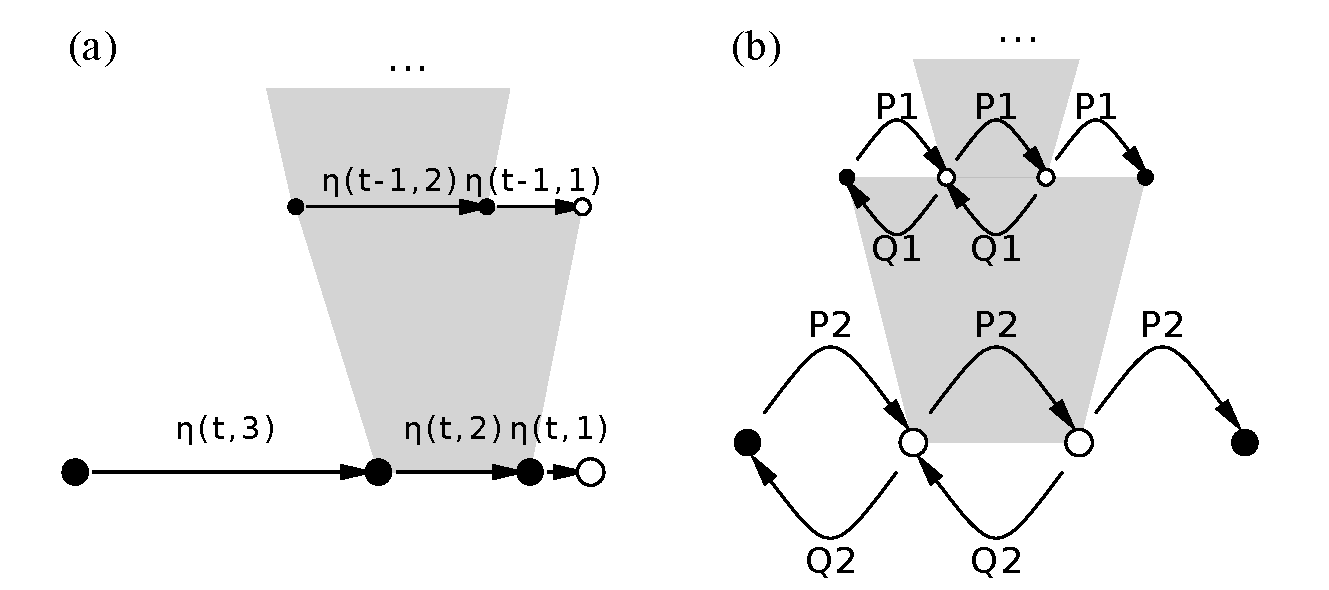
\includegraphics[width=0.88\columnwidth,trim={0 0cm 0 0cm},clip]{tradeoff.pdf}}
    \caption{(a) 广义自动微分中常见的Treeverse算法~\cite{Griewank1992},其中$\eta(\tau, \delta) \equiv \left(\begin{matrix} \tau + \delta \\ \delta \end{matrix}\right)=\frac{(\tau+\delta)!}{\tau!\delta!}$。(b) 可逆计算时空交换的Bennett算法。~\cite{Bennett1973,Levine1990} 其中,$P$和$Q$分别代表了计算和反计算。}\label{fig:tradeoff}
\end{figure}

可逆计算的优点是可以很方便的利用可逆性。


\begin{table}
    \centering
    \begin{tabularx}{0.6\textwidth}{cccc}\toprule
        \textbf{方法} & 时间最优 & 空间最优\\
        \hline
        检查点                           & $\bigO(T)/\bigO(TS)$   & $\bigO(T^2)/\bigO(S)$   \\
        可逆编程  & $\bigO(T)/\bigO(TS)$   & $\bigO(T(\frac{T}{S})^{0.585})/\bigO(S\log(\frac{T}{S}))$ \\
        \bottomrule
    \end{tabularx}
    \caption{$T$ and $S$ are the time and space of the original irreversible program. In the "Reverse computing" case, the reversibility of the original program is not utilized.}\label{tbl:timespace}
\end{table}

\begin{figure}[t]
\centering
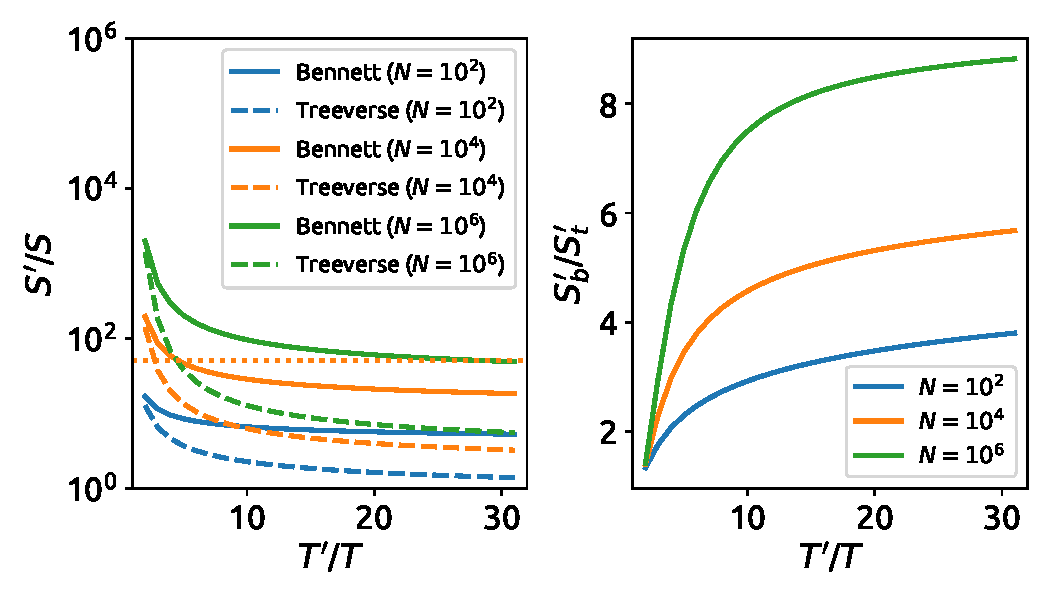
\includegraphics[width=0.8\columnwidth]{./fig1.pdf}
    \caption{为了回溯中间状态,时间和空间在两种最优时间-空间交换策略下的关系。(a) 固定横轴为状态回溯的计算时间与原函数计算时间的比值,对比再允许固定时间开销下,内存的额外开销。其中Bennett算法代表了可逆计算下的最优策略,而Treeverse则是传统计算允许的最优策略。(b) 对比Bennett算法与Treeverse算法空间开销的比值。\label{fig:timespace}} 
\end{figure}


\section{自动微分在物理中的应用}\label{sec:applications}
\vskip 1.55\baselineskip
\subsection{地震波的模拟}
后来在地震学的模拟中,它被用来微分地震波传播的过程~\cite{Symes2007}。

\vskip 1.55\baselineskip
%\subsection{热带(Tropical)张量网络求解自旋玻璃最优构型}
%热带张量网络是张量网络的一个特别的应用,它重新定义了张量中基础元素的代数为
%\begin{eqnarray}
%x \oplus y  = \max(x, y),\,\,\,\,\,\,\,\,\,\,\,\, \,\,\,\,
%x \odot y   =  x + y. \label{eq:max-sum-alg}
%\end{eqnarray}
%\begin{figure}[t]
%\centering
%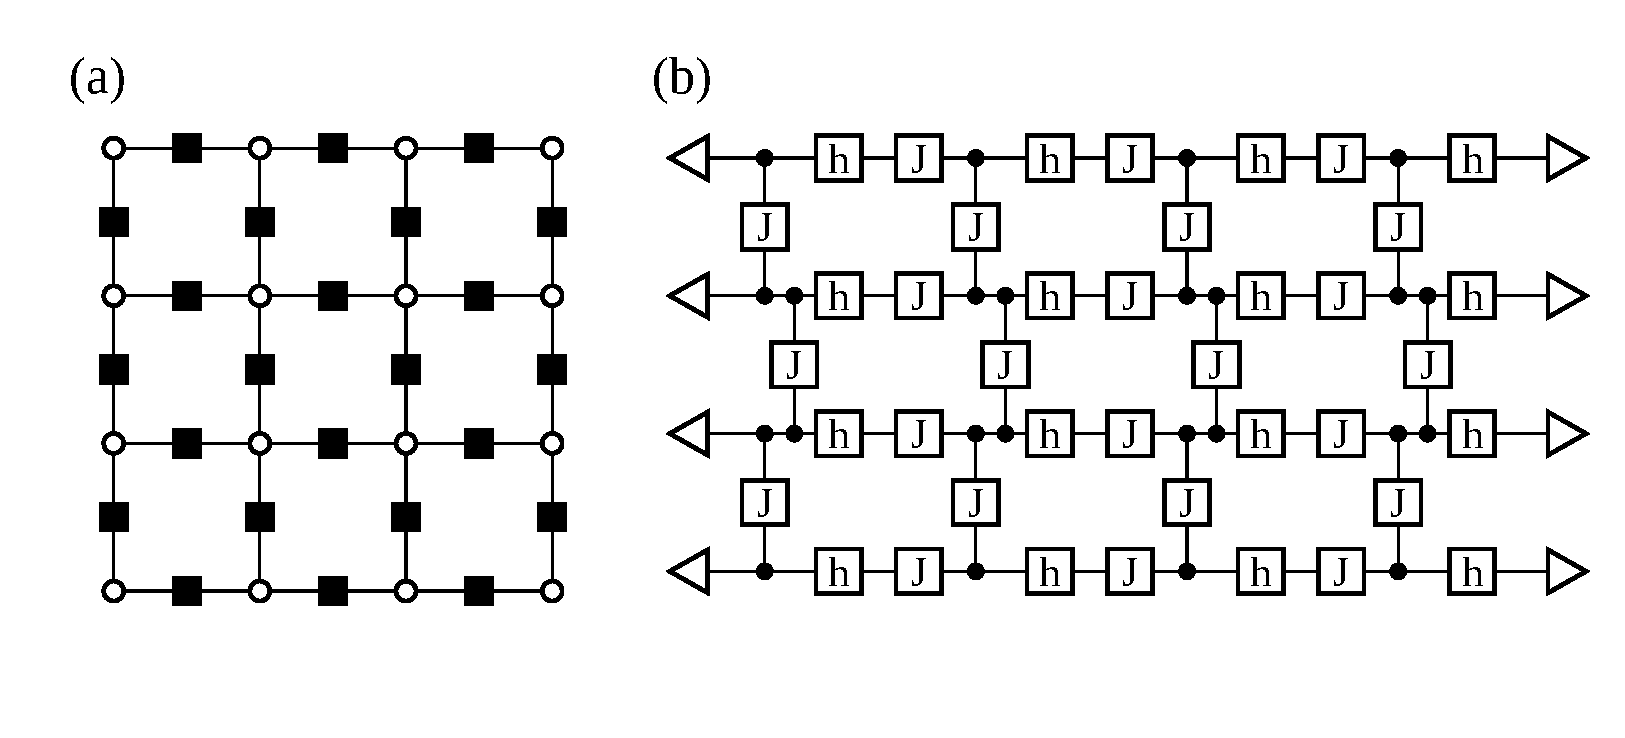
\includegraphics[width=\columnwidth]{./transform12.pdf}
    %\caption{正方晶格上的自旋玻璃问题,(a)对应的热带张量网络表示。(b)对应的“量子线路”表示。\label{fig:performance}} 
%\end{figure}
%如果我们将张量中的元素定义为自旋玻璃的耦合强度,我们就可以通过收缩这个张量结构得到自旋玻璃的最优构型。
%这个最优构型的能量表达式为
%\begin{equation}
    %E(\{\sigma\}) = \max\limits_{\sigma}-\sum_{i < j }J_{ij} \sigma_i \sigma_j  - \sum_i h_i \sigma_i,
%\label{eq:spinglassopt}
%\end{equation}
    %因此对它的微分就是。
%但是作了这样的替换,张量收缩的微分规则就发生了变换。

\section{结~~~~论}

\section*{致谢}

感谢北京大学力学系某某教授和某某博士以及某某的讨论.


\section*{附录A1}

标题排列和编号方式为A1, A2, A3.

\section*{附录A2}
%
%text text
%
%\section*{附录B1}
%%\section*{附录B2}
%
%text text
%
%\section*{致谢}
%
%text text

\bigskip
%\begin{footnotesize}

\bibliographystyle{apsrev4-1}
\bibliography{refs}

\newpage

\title{English Title $^{\ast}$}%{\efundlink}

\efund{Project supported by the State Key Development Program for Basic Research of China (Grant No. 2011CB00000), the National Natural Science Foundation of China (Grant Nos. 123456, 567890), and the National High Technology Research and Development Program of China (Grant No. 2011AA06Z000). \\}


\author{Guan Yun-Chang$^{1)2)}$ \quad  Liu Bei$^{1)\dag}$ \quad  Zhuge Liang$^{2)}$}

\email{aaa@bbb.ccc  }
%\email \emailddag


\eaddress{1)}{State Key Laboratory of Quantum Optics and Quantum Optics  Devices,
Institute of Opto-Electronics, Shanxi University, Taiyuan 030006, China}

\eaddress{2)}{Department of Physics, Tsinghua University, Beijing 100084, China}

\eabstract{}

\small  To determine the probe made of amino acids arranged in a linear chain and joined together by peptide bonds between the carboxyl and amino groups of adjacent amino acid residues. The sequence of amino acids in a protein is defined by a gene and encoded in the genetic code. This can happen either
before the protein is used in the cell, or as part of control mechanisms.

\ekeywords{Keyword1, Keyword2, Keyword3, Keyword4 \\}

\epacs{02.10.Yn, 33.15.Vb, 98.52.Cf, 78.47.dc}

\end{document}
